\chapter{Clasificación}
Se ha comprobado que usando regresión, se ha conseguido unos buenos modelos para predecir un valor \textbf{preciso} de la intención emprendedora media. El siguiente paso realizado ha sido el de \textbf{categorizar} el caso de regresión, obteniendo así clases del tipo \textit{intención emprendedora alta, baja o media}.\\
Hay que recordar que el resultado obtenido por el modelo de aprendizaje puede ser leído por personal no familiarizado con matemáticas o informática. Este enfoque lo que nos permite es usar una única variable como objetivo con los valores \textit{alto, bajo o alto}, siendo así más legible la salida del algoritmo.\\
\linebreak
Para categorizar los valores de predicción se ha establecido unos rangos y se van a transformar los valores de ese rango en las clases alta. media. y baja. Para establecer el rango, se ha ejecutado varias veces los algoritmos seleccionados y se han comparado las métricas obtenidas, usando unos rangos para establecer estas clases.\\
Los rangos que se han probado son:
\begin{itemize}
	\item $(4, 6, 7)$
	\item $(3.5, 5.5, 7)$
	\item $(3, 5, 7)$
\end{itemize}
Estas tuplas representan el valor usado para determinar el valor límite para clasificar una muestra como emprendimiento bajo, medio o alto (en ese orden).\\
\linebreak
\section{Rendimiento de modelos de clasificación}
Al igual que en los modelos de regresión, en clasificación se hace uso de métricas para ver el comportamiento de los modelos entrenados. A continuación se explica qué métricas se han usado:
\subsection{Accuracy}
Esta métrica mide el porcentaje de casos que el modelo ha clasificado correctamente.
\[
	accuracy(y,\hat{y})=\frac{1}{n_{samples}}\sum_{i=1}^{n_{samples}}1(\hat{y_i}=y_i)
\]

\subsection{Matriz de confusión y métricas}
Cada entrada $i.j$ de la matriz se define como el número de observaciones del grupo $i$ que han sido predichas como del grupo $j$. Un ejemplo de matriz de confusión para el problema que se esta tratando es:
\begin{figure}[H]
	\centering
	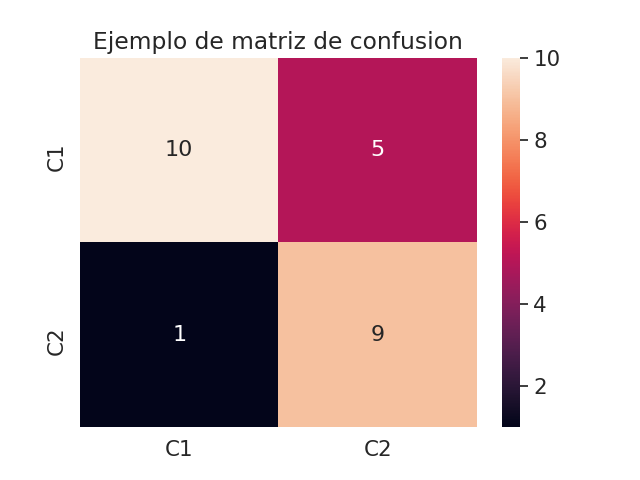
\includegraphics[scale=0.8]{conf_matrix.png}
	\caption{Ejemplo de matriz de confusión}
	\label{fig:conf_matrix}
\end{figure}
Aquí podemos ver cuantas muestras de una clase el modelo predijo como correctas (de la misma clase) y cuantas muestras de una clase predijo como erróneas (de distinta clase).\\
\linebreak
A partir de la matriz de confusión, se pueden sacar las siguiente métricas:
\[Precision = \frac{TP} {TP + FP}\]
\[Recall = \frac{TP}{TP + FN}\]
\[FPR = \frac{FP}{FP + TN}\]
\[ F1\_score = 2 \times \frac{Precision \times Recall}{Precision + Recall} \]
Intuitivamente, \textbf{Precision} mide la habilidad del modelo de no clasificar como \textbf{positiva} una muestra que es \textbf{negativa}, mientras que \textbf{Recall} mide la habilidad del modelo para clasificar bien todas las muestras positivas.\\
\linebreak
Cabe destacar que se han explicado para el caso de clasificación binaria, pero estas métricas se pueden extender para la clasificación multi-clase y multi-etiqueta.
\subsection{Curva ROC y AUC}
Partiendo de lo explicado sobre la matriz de confusión, la curva ROC (Receiver Operating Characteristic Curve) es un gráfico donde se representa el \textbf{FPR} (False Positive Rate) en el eje \textbf{X} y el \textbf{TPR} (True Positive Rate o Recall) en el eje \textbf{Y}. Se escogen estas métricas debido a la siguiente hipótesis:\\
A medida que incrementamos el ratio de verdaderos positivos, se va a incrementar el ratio de falsos positivos debido a que es más probable que el modelo clasifique como positivo una muestra que no es positiva.
\begin{figure}[H]
	\centering
	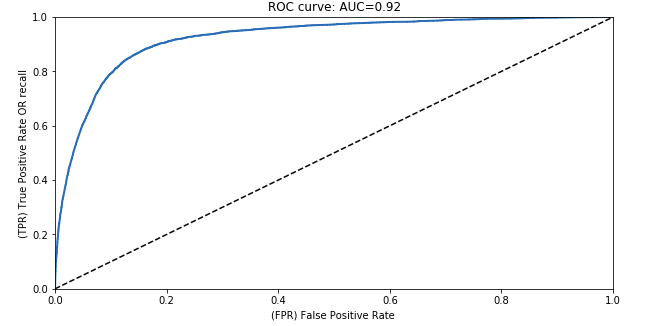
\includegraphics[scale=0.5]{roc}
	\caption{Ejemplo de curva ROC}
	\label{fig:roc}
\end{figure}
Lo ideal, es que la figura se acerque a la esquina superior izquierda lo máximo posible, ya que implicaría que se esta clasificando como correctos todas las muestras positivas y ninguna muestra negativa se está clasificando como positiva.\\
Se puede usar el área bajo la curva como una métrica para comprobar como de bueno es el modelo. Esta métrica se conoce como \textbf{AUC} (Area Under Curve).\\
\linebreak
Al igual que en regresión (\ref{sec:validation}-\nameref{sec:validation}), se ha usado la técnica de \textit{k-fold validation} para validar el rendimiento de los modelos entrenados.
\section{Modelos de clasificación}
Para clasificación, se van a usar unicamente aquellos modelos que se ha demostrado empíricamente en la sección \ref{sec:algoritmos}-\nameref{sec:algoritmos} que han tenido un buen desempeño. Por tanto se van a usar Árboles de Decisión, Random Forest y SVM.
\subsection{Árboles de Decisión}
En esta sección se va a exponer los resultados obtenidos en clasificación usando \textbf{Árboles de Decisión}.\\
La siguiente tabla expone los resultados obtenidos:
\begin{figure}[H]
	\centering
	\includegraphics[scale=0.7]{src/dt_cmp_val_metrics}
	\caption{Comparación en conjunto de validación}
	\label{fig:dtre_class_val}
\end{figure}
\begin{figure}[H]
	\centering
	\includegraphics[scale=0.7]{src/dt_cmp_test_metrics}
	\caption{Comparación en conjunto de test}
	\label{fig:dtre_class_testl}
\end{figure}
A continuación, las tablas con los resultados de las métricas y las matrices de confusión obtenidas por los Árboles de decisión usando la categorización usando los rangos $(3.5,5.5,7)$ y $(4,6,7)$
\subsubsection*{Rango $(3.5,5.5,7)$}
\begin{table}[H]
	\centering
	\begin{tabular}{|c|c|c|c|c}
		\cline{1-4}
		FOLD   & F1 Score & AUC Score & Accuracy \\ \cline{1-4}
		Fold 0 & 0.684    & 0.822     & 0.713    \\ \cline{1-4}
		Fold 1 & 0.699    & 0.881     & 0.725    \\ \cline{1-4}
		Fold 2 & 0.691    & 0.84      & 0.713    \\ \cline{1-4}
		Fold 3 & 0.664    & 0.833     & 0.701    \\ \cline{1-4}
		Fold 4 & 0.753    & 0.869     & 0.768    \\ \cline{1-4}
		Fold 5 & 0.698    & 0.849     & 0.724    \\ \cline{1-4}
		Train  & 0.781    & 0.909     & 0.794    \\ \cline{1-4}
		Test   & 0.701    & 0.843     & 0.715    \\ \cline{1-4}
	\end{tabular}
	\caption{Valores de métricas obtenidos usando rango $(3.5,5.5,7)$}
\end{table}

\begin{figure}[H]
	\centering
	\includegraphics[scale=0.5]{src/confusion_matrix_dtree_classification_3-5_5-5_7.png}
	\caption{Matriz de confusión para Árboles de Decisión usando $(3.5,5.5,7)$}
	\label{fig:confusion_matrix_dtree1}
\end{figure}
\subsubsection*{Rango $(4,6,7)$}
\begin{table}[H]
	\centering
	\begin{tabular}{|c|c|c|c|c}
		\cline{1-4}
		FOLD   & F1 Score & AUC Score & Accuracy \\ \cline{1-4}
		Fold 0 & 0.709    & 0.861     & 0.705    \\ \cline{1-4}
		Fold 1 & 0.686    & 0.828     & 0.681    \\ \cline{1-4}
		Fold 2 & 0.698    & 0.842     & 0.697    \\ \cline{1-4}
		Fold 3 & 0.715    & 0.855     & 0.709    \\ \cline{1-4}
		Fold 4 & 0.69     & 0.836     & 0.688    \\ \cline{1-4}
		Fold 5 & 0.7      & 0.844     & 0.696    \\ \cline{1-4}
		Train  & 0.752    & 0.89      & 0.746    \\ \cline{1-4}
		Test   & 0.721    & 0.867     & 0.72     \\ \cline{1-4}
	\end{tabular}
	\caption{Valores de métricas obtenidos usando rango $(4,6,7)$}
\end{table}

\begin{figure}[H]
	\centering
	\includegraphics[scale=0.5]{src/confusion_matrix_dtree_classification_4_6_7}
	\caption{Matriz de confusión para Árboles de Decisión usando $(4,6,7)$}
	\label{fig:confusion_matrix_dtree2}
\end{figure}
\pagebreak
\subsection{Random Forest}
En esta sección se va a exponer los resultados obtenidos en clasificación usando \textbf{Random Forest}.
A continuación se muestran una serie de gráficos comparando las distintas métricas que se han seleccionado:
\begin{figure}[H]
	\centering
	\includegraphics[scale=0.5]{src/rf_class_cmp_val_metrics}
	\caption{Comparación en conjunto de validación}
	\label{fig:rf_class_cmp_val}
\end{figure}

\begin{figure}[H]
	\centering
	\includegraphics[scale=0.5]{src/rf_class_cmp_test_metrics}
	\caption{Comparación en conjunto de test}
	\label{fig:rf_class_cmp_test}
\end{figure}
En las secciones siguientes, se va a mostrar las tablas con los valores de métricas obtenidas por Random Forest y las matrices de confusión correspondientes.
\subsubsection*{Rango $(3,5,7)$}
\begin{table}[H]
	\centering
	\begin{tabular}{|c|c|c|c|c}
		\cline{1-4}
		FOLD   & F1 Score & AUC Score & Accuracy \\ \cline{1-4}
		Fold 0 & 0.694    & 0.858     & 0.721    \\ \cline{1-4}
		Fold 1 & 0.755    & 0.898     & 0.769    \\ \cline{1-4}
		Fold 2 & 0.699    & 0.883     & 0.717    \\ \cline{1-4}
		Fold 3 & 0.693    & 0.867     & 0.709    \\ \cline{1-4}
		Fold 4 & 0.748    & 0.892     & 0.776    \\ \cline{1-4}
		Fold 5 & 0.718    & 0.88      & 0.738    \\ \cline{1-4}
		Train  & 0.993    & 1.0       & 0.994    \\\cline{1-4}
		Test   & 0.739    & 0.885     & 0.761    \\ \cline{1-4}
	\end{tabular}
	\caption{Valores de métricas obtenidos usando rango $(3,5,7)$}
\end{table}
\begin{figure}[H]
	\centering
	\includegraphics[scale=0.5]{src/confusion_matrix_rf_class_3_5_7.png}
	\caption{Matriz de confusión para Random Forest usando $(3,5,7)$}
	\label{fig:confusion_matrix_rf1}
\end{figure}

\subsection*{Rango $(4,6,7)$}
\begin{table}[H]
	\centering
	\begin{tabular}{|c|c|c|c|c}
		\cline{1-4}
		FOLD   & F1 Score & AUC Score & Accuracy \\ \cline{1-4}
		Fold 0 & 0.702    & 0.887     & 0.701    \\  \cline{1-4}
		Fold 1 & 0.72     & 0.884     & 0.713    \\  \cline{1-4}
		Fold 2 & 0.763    & 0.903     & 0.765    \\  \cline{1-4}
		Fold 3 & 0.747    & 0.891     & 0.745    \\  \cline{1-4}
		Fold 4 & 0.703    & 0.868     & 0.696    \\  \cline{1-4}
		Fold 5 & 0.727    & 0.887     & 0.724    \\  \cline{1-4}
		Train  & 0.998    & 1.0       & 0.998    \\ \cline{1-4}
		Test   & 0.748    & 0.901     & 0.746    \\ \cline{1-4}
	\end{tabular}
	\caption{Valores de métricas obtenidos usando rango $(4,6,7)$}
\end{table}
\begin{figure}[H]
	\centering
	\includegraphics[scale=0.5]{src/confusion_matrix_rf_class_4_6_7.png}
	\caption{Matriz de confusión para Random Forest usando $(4,6,7)$}
	\label{fig:confusion_matrix_rf2}
\end{figure}
\pagebreak
\subsection{Support Vector Machines}
En esta sección se va a exponer los resultados obtenidos en clasificación usando \textbf{SVM}.
A continuación se muestran una serie de gráficos comparando las distintas métricas que se han seleccionado:
\begin{figure}[H]
	\centering
	\includegraphics[scale=0.5]{src/svc_cmp_val_metrics.png}
	\caption{Comparación en conjunto de validación}
	\label{fig:svc_class_cmp_val}
\end{figure}

\begin{figure}[H]
	\centering
	\includegraphics[scale=0.5]{src/svc_cmp_test_metrics.png}
	\caption{Comparación en conjunto de test}
	\label{fig:svc_class_cmp_test}
\end{figure}
En las secciones siguientes, se va a mostrar las tablas con los valores de métricas obtenidas por SVM y las matrices de confusión correspondientes.
\subsubsection*{Rango $(3.5,5.5,7)$}
\begin{table}[H]
	\centering
	\begin{tabular}{|c|c|c|c|c}
		\cline{1-4}
		FOLD   & F1 Score & AUC Score & Accuracy \\ \cline{1-4}
		Fold 0 & 0.682    & 0.846     & 0.717    \\ \cline{1-4}
		Fold 1 & 0.713    & 0.887     & 0.753    \\ \cline{1-4}
		Fold 2 & 0.729    & 0.899     & 0.749    \\ \cline{1-4}
		Fold 3 & 0.698    & 0.861     & 0.713    \\ \cline{1-4}
		Fold 4 & 0.735    & 0.91      & 0.772    \\ \cline{1-4}
		Fold 5 & 0.711    & 0.881     & 0.741    \\ \cline{1-4}
		Train  & 0.928    & 0.989     & 0.933    \\ \cline{1-4}
		Test   & 0.712    & 0.887     & 0.742    \\ \cline{1-4}
	\end{tabular}
	\caption{Valores de métricas obtenidos usando rango $(3.5,5.5,7)$}
\end{table}
\begin{figure}[H]
	\centering
	\includegraphics[scale=0.5]{src/confusion_matrix_svc_3-5_5-5_7.png}
	\caption{ confusión para SVM usando $(3.5,5.5,7)$}
	\label{fig:confusion_matrix_svm1}
\end{figure}

\subsubsection*{Rango $(4,6,7)$}
\begin{table}[H]
	\centering
	\begin{tabular}{|c|c|c|c|c}
		\cline{1-4}
		FOLD   & F1 Score & AUC Score & Accuracy \\ \cline{1-4}
		Fold 0 & 0.65     & 0.856     & 0.649    \\  \cline{1-4}
		Fold 1 & 0.702    & 0.886     & 0.705    \\  \cline{1-4}
		Fold 2 & 0.742    & 0.88      & 0.745    \\  \cline{1-4}
		Fold 3 & 0.739    & 0.888     & 0.741    \\  \cline{1-4}
		Fold 4 & 0.681    & 0.862     & 0.676    \\  \cline{1-4}
		Fold 5 & 0.703    & 0.874     & 0.703    \\  \cline{1-4}
		Train  & 0.918    & 0.991     & 0.917    \\  \cline{1-4}
		Test   & 0.714    & 0.881     & 0.718    \\  \cline{1-4}
	\end{tabular}
	\caption{Valores de métricas obtenidos usando rango $(4,6,7)$}
\end{table}
\begin{figure}[H]
	\centering
	\includegraphics[scale=0.5]{src/confusion_matrix_svc_4_6_7.png}
	\caption{Matriz de confusión para SVM usando $(4,6,7)$}
	\label{fig:confusion_matrix_svc2}
\end{figure}

\subsection{Análisis de resultados}
Como se puede apreciar, ninguno de los algoritmos no han tenido problemas clasificando la clase \textbf{IEAlta}, clasificando correctamente más del $80\%$ de las instancias de esta clase.
Los algoritmos han tenido más problemas a la hora de clasificar correctamente la clase \textbf{IEBaja}, clasificando correctamente solo el $50\%$. Volviendo a la figura \ref{tab:ocurrencia_valores} donde se mostraba el conteo de clases, se puede apreciar que la clase formada por los valores más bajos tiene una menor cantidad de muestras, explicando así que los algoritmos fallen más comúnmente en estas clases, clasificando una gran parte como \textbf{IEMedia} (tiene sentido ya que es la clase más 'cercana').
\linebreak
Respecto al rendimiento se puede observar como los modelos basados en árboles de decisión siguen comportándose correctamente, siendo Random Forest el que mejor resultados obtuvo. \\
SVM siguió comportándose de manera correcta, obteniendo unos resultados ligeramente peores que Random Forest pero mejores que Árboles de decisión.
\linebreak
Por ultimo, se puede observar revisando los resultados que el rango de conversión que mejor ha funcionado para Random Forest y Árboles de decisión ha sido:
\begin{enumerate}
    \item Reemplazar por \textit{IEBAJA} aquellos valores de \textit{IEMEdia} menores a 4.
    \item Reemplazar por \textit{IEMEDIA} aquellos valores de \textit{IEMEdia} menores a 6.
    \item Reemplazar por \textit{IEALTA} aquellos valores de \textit{IEMEdia} menores a 7.
\end{enumerate}
Mientras que para SVM ha sido:
\begin{enumerate}
    \item Reemplazar por \textit{IEBAJA} aquellos valores de \textit{IEMEdia} menores a 3.5.
    \item Reemplazar por \textit{IEMEDIA} aquellos valores de \textit{IEMEdia} menores a 5.5.
    \item Reemplazar por \textit{IEALTA} aquellos valores de \textit{IEMEdia} menores a 7.
\end{enumerate}

\begin{figure}[H]
    \centering
    \includegraphics[scale=0.5]{src/class_comp_val_metrics.png}
    \caption{Comparación del rendimiento en el conjunto de validación}
    \label{fig:class_cmp_val}
\end{figure}
\begin{figure}[H]
    \centering
    \includegraphics[scale=0.5]{src/class_comp_test_metrics.png}
    \caption{Comparación del rendimiento en el conjunto de test}
    \label{fig:class_cmp_test}
\end{figure}
Cabe destacar que estos resultados no son comparables, ya que el conjunto de datos sobre el que se ha entrenado los algoritmos es distinto.
Una causa por la que  SVM rindió mejor en el conjunto $(3.5,5.5,7)$ es que como el conjunto de datos tiene una mayor cantidad de valores en el rango medio, SVM dispone de una mayor cantidad de vectores soporte y facilitando el encontrar un hiperplano que divida mejor los datos.
\section{Segunda iteración}
\label{sec:ord}
Como se puede observar, las resultados han sido buenos, teniendo la mayor parte de algoritmos un comportamiento similar al observado en regresión (Random Forest ha sido el modelo que mejor ha funcionado, mientras que Árboles de Decisión y SVM han tenido un comportamiento similar).\\
La opción por la que se ha optado de \textbf{categorizar} el problema de regresión de la forma en la que se ha explicado tiene un inconveniente: No se está teniendo en cuenta el \textbf{orden} de las clases, ya que el algoritmo de clasificación trata las distintas clases como un conjunto de valores sin orden.
Para mejorar este comportamiento, se va a optar por seguir el enfoque explicado en el artículo \textit{A Simple Approach to Ordinal Classification}. La propuesta es la siguiente:
En lugar de clasificar $k$ clases, se van a entrenar $k-1$ clasificadores binarios donde la variable objetivo del modelo $M_i$ representa la \textbf{probabilidad} de que la clase sea mayor (según el orden) que la clase $K_i$. El siguiente ejemplo ayuda a explicar este enfoque:\\
\linebreak
Se quiere predecir el ranking (de 1 a 5) que un usuario le va a dar a una película. Para ello se van a entrenar los siguientes $4$ modelos:
\begin{enumerate}
    \item El primer modelo calcula la probabilidad de que el ranking predicho sea mayor que 1.
    \item El segundo modelo calcula la probabilidad de que el ranking predicho sea mayor que 2.
    \item El tercer modelo calcula la probabilidad de que el ranking predicho sea mayor que 3.
    \item El cuarto modelo calcula la probabilidad de que el ranking predicho sea mayor que 4.
\end{enumerate}
Una vez que se han calculado las probabilidades, el modelo escoge aquella clase con mayor probabilidad. Obviamente, es muy importante optar por este enfoque que el modelo seleccionado sea capaz de obtener la \textbf{probabilidad} de que una muestra pertenezca a una clase. Los modelos seleccionados en este capítulo son capaces de obtener las probabilidades de clase.
\linebreak
Este tipo de algoritmo no esta implementado en la librería Scikit-Learn, pero esta provee de las herramientas necesarias para construir modelos personalizados y que sean compatibles con el resto de utilidades que la librería ofrece. Este proceso se va a explicar en la sección \ref{sec:sftw}-\nameref{sec:sftw}.\\
\subsection{Resultados}
En esta sección se van a presentar una comparativa entre los resultados obtenidos por los algoritmos de clasificación ordinal desarrollados y los resultados obtenidos por los algoritmos nativos que se han usado. Para facilitar la comparación, se han elegido unicamente los conjuntos de datos $(3.5,5.5,7)$  y $(4,6,7)$, puesto que han sido los conjuntos de datos en los que los algoritmos han mostrado diferencias en el rendimiento.

\subsubsection*{Árboles de decisión}
\label{sec:ord_cmp_dt}
A continuación se muestran la comparativa para el conjunto $(3.5,5.5,7)$ entre el algoritmo de clasificación ordinal implementando  (usando Árboles de Decisión) y el algoritmo de clasificación estándar:
\begin{figure}[H]
    \centering
    \includegraphics[scale=0.5]{src/dt_ordinal_cmp_3_5_val_metrics.png}
    \caption{Comparación en validación para el conjunto  $(3.5,5.5,7)$ }
    \label{fig:dt_ordin_val_cmp_1}
\end{figure}
\begin{figure}[H]
    \centering
    \includegraphics[scale=0.5]{src/dt_ordinal_cmp_3_5_test_metrics.png}
    \caption{Comparación en test para el conjunto  $(3.5,5.5,7)$}
    \label{fig:dt_ordint_test_cmp_1}
\end{figure}
A
Las gráficas siguientes muestran la comparativa para el conjunto $(4,6,7)$ entre el algoritmo de clasificación ordinal implementando  (usando Árboles de Decisión) y el algoritmo de clasificación estándar:
\begin{figure}[H]
    \centering
    \includegraphics[scale=0.5]{src/dt_ordinal_cmp_4_6_val_metrics.png}
    \caption{Comparación en validación para el conjunto $(4,6,7)$}
    \label{fig:dt_ordin_val_cmp_2}
\end{figure}
\begin{figure}[H]
    \centering
    \includegraphics[scale=0.5]{src/dt_ordinal_cmp_4_6_test_metrics.png}
    \caption{Comparación en test para el conjunto  $(4,6,7)$}
    \label{fig:dt_ordint_test_cmp_2}
\end{figure}

Se puede observar que los resultados obtenidos usando una clasificación estándar ha sido ligeramente mejor que usando el algoritmo de clasificación ordinal. Parece que para árboles de decisión, en este caso, el orden de las clases no ha tenido una relevancia
\subsubsection*{Random Forest}
\label{sec:ord_cmp_rf}
A continuación se muestran la comparativa para el conjunto $(3.5,5.5,7)$ entre el algoritmo de clasificación ordinal implementando  (usando Random Forest)  y el algoritmo de clasificación estándar:\\
\begin{figure}[H]
    \centering
    \includegraphics[scale=0.5]{src/rf_ordinal_cmp_3_5_val_metrics.png}
    \caption{Comparación en validación para el conjunto  $(3.5,5.5,7)$ }
    \label{fig:rf_ordin_val_cmp_1}
\end{figure}
\begin{figure}[H]
    \centering
    \includegraphics[scale=0.5]{src/rf_ordinal_cmp_3_5_test_metrics.png}
    \caption{Comparación en test para el conjunto  $(3.5,5.5,7)$}
    \label{fig:rf_ordint_test_cmp_1}
\end{figure}
Las gráficas siguientes muestran la comparativa para el conjunto $(4,6,7)$ entre el algoritmo de clasificación ordinal implementando  (usando Random Forest) y el algoritmo de clasificación estándar:
\begin{figure}[H]
    \centering
    \includegraphics[scale=0.5]{src/rf_ordinal_cmp_4_6_val_metrics.png}
    \caption{Comparación en validación para el conjunto $(4,6,7)$}
    \label{fig:rf_ordin_val_cmp_2}
\end{figure}
\begin{figure}[H]
    \centering
    \includegraphics[scale=0.5]{src/rf_ordinal_cmp_4_6_test_metrics.png}
    \caption{Comparación en test para el conjunto  $(4,6,7)$}
    \label{fig:rf_ordint_test_cmp_2}
\end{figure}


\subsubsection*{Support Vector Machine}
\label{sec:ord_cmp_svm}
A continuación se muestran la comparativa para el conjunto $(3.5,5.5,7)$ entre el algoritmo de clasificación ordinal implementando  (usando Random Forest)  y el algoritmo de clasificación estándar:
\begin{figure}[H]
    \centering
    \includegraphics[scale=0.5]{src/svc_ordinal_cmp_3_5_val_metrics.png}
    \caption{Comparación en validación para el conjunto  $(3.5,5.5,7)$ }
    \label{fig:svc_ordin_val_cmp_1}
\end{figure}
\begin{figure}[H]
    \centering
    \includegraphics[scale=0.5]{src/svc_ordinal_cmp_3_5_test_metrics.png}
    \caption{Comparación en test para el conjunto  $(3.5,5.5,7)$}
    \label{fig:svc_ordin_test_cmp_1}
\end{figure}
Las gráficas siguientes muestran la comparativa para el conjunto $(4,6,7)$ entre el algoritmo de clasificación ordinal implementando  (usando SVM) y el algoritmo de clasificación estándar:
\begin{figure}[H]
    \centering
    \includegraphics[scale=0.5]{src/svc_ordinal_cmp_4_6_val_metrics.png}
    \caption{Comparación en validación para el conjunto $(4,6,7)$}
    \label{fig:svc_ordin_val_cmp_2}
\end{figure}
\begin{figure}[H]
    \centering
    \includegraphics[scale=0.5]{src/svc_ordinal_cmp_4_6_test_metrics.png}
    \caption{Comparación en test para el conjunto  $(4,6,7)$}
    \label{fig:svc_ordin_test_cmp_2}
\end{figure}
\subsection{Análisis de resultados}
Comenzando por \nameref{sec:ord_cmp_dt}, se puede apreciar como este algoritmo ha sido más robusto a la hora de clasificar de manera tradicional, ya que en este caso, el algoritmo de clasificación ordinal ha rendido ligeramente peor. Llama la atención que ha sido el \textbf{único} de los modelos seleccionados que ha rendido mejor el algoritmo de clasificación clásico. Este comportamiento puede darse a que debido que se está entrenando varios modelos para predecir la salida (explicado en \ref{sec:ord}-\nameref{sec:ord}) y siendo los árboles de decisión (como ya se ha visto en secciones anteriores) muy sensibles al ruido, la posibilidad de entrenar un modelo que induzca a error es alta,. Dado que el algoritmo implementado para la clasificación ordinal elige la salida que tenga una mayor probabilidad, es la causa probable de este comportamiento.\\
\linebreak
En cuanto a Random Forest, como se puede ver en las gráficas expuestas en \ref{sec:ord_cmp_rf}-\nameref{sec:ord_cmp_rf}, se ha conseguido una ligera mejora en las métricas usando el algoritmo de clasificación ordinal. A diferencia de Árboles de decisión, se ha podido apreciar en secciones anteriores como Random Forest es mas tolerante al ruido, eso hace que para usarlo como clasificador ordinal sea una buena opción.\\
\linebreak
Por ultimo, respecto a SVM, se ha apreciado una ligera mejora usando el algoritmo de clasificación ordinal. Al igual que Random Forest, se ha podido comprobar empíricamente que SVM ha sido tolerante con el ruido del conjunto de datos, por lo que hace que sea un algoritmo bueno a la hora de realizar la clasificación ordinal usando este conjunto de datos.\\
\linebreak
Generalmente, los algoritmos que han probado ser más sensibles al ruido han tenido un menor desempeño que algoritmos con mejor tolerancia a error. Random Forest en este caso, sigue siendo el algoritmo con mejores resultados, mientras que algoritmos más simples como Árboles de Decisión han tenido un rendimiento menor.
